%% ---------------------------------------------------------------------------
%% CAIN 2027, research track. Double-anonymous, 10 pages + 2 of references.
%% Deadline: 30 October 2026, firm.
%%
%% Self-contained on purpose: the algebra and its proof are restated rather
%% than cited, so this paper stands alone. The companion submission elsewhere
%% covers the vocabulary alignment and the archive study, neither of which
%% appears here; this paper's contribution is the system and the cost of
%% running it.
%% ---------------------------------------------------------------------------
\documentclass[10pt,conference]{IEEEtran}
\IEEEoverridecommandlockouts

\usepackage{cite}
\usepackage{amsmath,amssymb}
\usepackage{booktabs}
\usepackage{url}
\usepackage{algorithm}
\usepackage{algpseudocode}
\usepackage{listings}
\usepackage{tikz}
\usetikzlibrary{arrows.meta,positioning,shapes.geometric}
\usepackage{pgfplots}
\pgfplotsset{compat=1.18}
\usepackage[hidelinks]{hyperref}

%% The worked example shows real JSON-LD, so the listing style has to be
%% readable at this size without colour.
\lstdefinestyle{jsonld}{
  basicstyle=\ttfamily\scriptsize,
  columns=fullflexible,
  breaklines=true,
  showstringspaces=false,
  frame=none,
  aboveskip=2pt,
  belowskip=2pt,
}

%% Anything still to be filled from the cluster campaign is wrapped in this, so
%% an unverified number cannot reach a draft unnoticed. It must not appear in
%% the submitted version.
\newcommand{\pending}[1]{\textbf{[PENDING: #1]}}

\newcommand{\repourl}{\url{https://anonymous.4open.science/r/sac-154B/}}

\begin{document}

\title{Policy-Aware Admission Control for Federated Learning}

\author{\IEEEauthorblockN{Anonymous Author(s)}}

\maketitle

\begin{abstract}
A federated learning system decides which clients take part in training, and
every selection strategy we are aware of decides this on statistical grounds:
how much data a client holds, how fast it is, how useful its gradients appear.
None of them asks whether the resulting model may lawfully be used. That
question has an answer only once the conditions attached to every contributor's
data have been combined, and combining them is not a matter of collecting
documents, because conditions of use interact. We present an admission control
mechanism that treats those conditions as a first-class input to the training
pipeline. Its basis is a composition algebra for a fragment of ODRL, together
with a proof that capability is anti-monotone in the contributor set, so that
admitting a client can only narrow what the group may do with the model it
produces. Anti-monotonicity makes the resulting search downward closed and therefore prunable. That is what allows the check to run before the first training round, and not as an audit afterwards. We implement this as a
Flower strategy that collects declarations from the connected nodes, composes
them, fixes membership before round one, refuses to start when an obligation
has not been discharged, re-checks consent between rounds, and emits a model
bundle carrying the agreement it was trained under. Because the policy filter
leaves many admissible groups and says nothing about which of them trains best,
we pair it with a second stage that ranks the survivors by a short exploratory
run. We measure what that costs on an exhaustively trained lattice: every one
of the 1023 candidate consortia, at 20 federations, with five replicates each,
so that a candidate is chosen on one training run and scored on others. Around
eight of twenty rounds turns out to be \emph{equivalent} to training every
candidate to completion, in the sense that the paired difference between them
is smaller than the full budget's own distance from the truth, at two fifths of the compute. The heuristic of admitting every permitted contributor gives up
1.72 percentage points. We also report three training-free estimators that do
not work, one of which anti-correlates with accuracy, because they are the
reason the second stage has to train at all.
\end{abstract}

\begin{IEEEkeywords}
federated learning, usage control, admission control, client selection, ODRL,
policy composition, AI engineering
\end{IEEEkeywords}

%% ===========================================================================
\section{Introduction}
\label{sec:intro}

A federated learning system has to decide who trains. The server makes this decision, usually once per round, and there is a large literature on how to make it well. Participants can be ranked by the volume of data they hold, by the staleness of their updates, by their expected latency, or by a statistical utility derived from their local loss. What these strategies have in common is
that they are all concerned with the quality of the model that results. None of
them is concerned with whether that model may be used.

The question is not rhetorical. When several institutions contribute data to a
shared model, each of them attaches conditions to the data it contributes, and
those conditions bind the artefacts derived from it. A hospital may permit its
records to be used for cancer research but not for commercial purposes. Another may permit commercial use but require that any derived model be published. A third may permit neither and require that results be returned to it before
release. A model trained on all three is a derivative of all three sets of
terms simultaneously, and what may be done with it is whatever all three allow
at once. That may be nothing.

This is a systems problem and not a legal one, and the reason is timing. The
conditions are known before training begins, they are machine-readable in a
growing number of real settings, and the composition that determines the
group's rights is computable. A system that does not compute it has to discover the answer afterwards, once the compute has already been spent. At that point the discovery cannot be acted upon. The model exists, it is a derivative of terms that forbid the intended use, and no amount of retraining on a subset undoes the fact that the weights were seen. A system that does compute it can decline to
start.

What makes the check tractable is a property of composition itself. Consider
three institutions declaring the purposes for which their data may be used, such
that contributor A permits cancer research or method development, contributor B
permits neurological research or method development, and contributor C permits
cancer or neurological research. Any two of them share a purpose, so a server
that assessed each candidate separately against its own research question would
conclude that every one of them is acceptable. All three together share none.
Compatibility is not transitive, and a system that checks members one at a time
proves nothing about the group.

The same example shows the way out. Because the group's permissions are the
intersection of its members' permissions, admitting a member can never add a
permission that was not already there. Capability therefore shrinks as the group
grows, which makes the family of admissible groups downward closed, and a
downward closed family can be searched by generating candidates only from
admissible smaller ones. The search over subsets that looks exponential is
prunable for the same reason that made the problem hard.

This paper is about what follows from building that into a federated learning
server. We make four contributions.

First, a composition algebra for a fragment of ODRL, with a proof that
capability is anti-monotone in the contributor set. We restate the algebra here in full instead of citing it, so that the system can be read without reference to
anything else, and the proof is what licenses the pruning.

Second, a Flower strategy, \texttt{PolicyAwareFedAvg}, in which admission is a
pure function of the declarations the nodes send. The server states what the
federation needs to be able to do, collects declarations, composes them,
searches for a group whose combined terms grant the requirement, and trains only
on that group. It refuses to begin when an obligation cannot be discharged by training and no evidence is given that somebody discharged it some other way. Between rounds it re-asks every active node for its terms, so that membership can shrink when consent is withdrawn. At the end it writes the trained weights alongside the agreement they were produced under.

Third, a two-stage selection pipeline. The policy filter decides which groups
are admissible and is silent on which of them trains best, so the second stage
ranks the survivors by a short exploratory run and continues only the leaders.
We measure the trade-off this offers on an exhaustively trained lattice.

Fourth, a negative result. Three training-free estimators of group utility, one
of them novel, all fail to rank candidates usefully, and the novel one
anti-correlates with accuracy. We report this because it is the argument for the
shape of the second stage: if a cheap estimator worked, the system would not
need to train anything to rank.

Section~\ref{sec:related} positions the work. Section~\ref{sec:algebra}
presents the algebra and the property the system rests on.
Section~\ref{sec:system} describes the server. Section~\ref{sec:twostage}
describes the second stage. Section~\ref{sec:eval} reports what it costs and
what it recovers, and Section~\ref{sec:discussion} discusses what the results
do and do not establish.

%% ===========================================================================
\section{Research Context}
\label{sec:related}

This section reviews the three bodies of work that our contribution sits
between. The first is concerned with choosing clients well. The second is
concerned with expressing conditions of use. The third is concerned with
recording what a model was built from. We then explain what none of them
provides.

\subsection{Client Selection in Federated Learning}

Which clients take part in a round is a well-studied lever. Federated
averaging~\cite{fedavg} samples participants uniformly at random. A good deal
of later work improves on that by selecting on some signal that correlates with
the value of a client's contribution.

Oort~\cite{oort} is a representative example. It ranks participants by a
statistical utility derived from their local training loss, combined with a
measure of how quickly each one can finish a round, and it reports large
reductions in the time needed to reach a target accuracy. A second family of
methods attributes a model's performance among the clients that produced it.
Data Shapley~\cite{datashapley} is the best known of these. Such methods can be
used to select clients, but their cost grows very quickly as the number of
participants rises. Other strategies select clients in order to correct for
differences in their data distributions, to keep updates from becoming stale,
or to respect the energy budget of a device.

All of these methods have one thing in common. They are concerned with the
quality of the model that will result. None of them is concerned with whether
that model may be used once it exists. Our mechanism therefore does not compete
with them. It runs before them, and it answers a different question: which
groups of clients are permitted at all. A statistical selector then chooses
among the groups that our mechanism allows. We keep the two apart in our
implementation for this reason, and the second of them could be replaced by any
of the methods above without changing the first.

\subsection{Expressing Conditions of Use}

The Open Digital Rights Language~\cite{odrl-model,odrl-vocab} is a W3C
Recommendation. It provides a model of permissions, prohibitions, duties and
constraints over assets, and it is serialised as linked data. ODRL describes
what may be done with an asset. It does not say what happens when several
policies have to hold at the same time, and it has no vocabulary for the
artefact that training produces.

In September 2026 the ODRL community published a draft profile for
AI~\cite{odrl-ai}. The profile introduces actions that are specific to AI
workflows, among them \emph{ai-training} for fine-tuning and
\emph{ai-augment} for retrieval and grounding. This makes the question of
derived artefacts more pressing and not less, because those two actions are
exactly how private data is used to adapt a model today.

Licence composition is mature in software. SPDX~\cite{spdx} defines licence
expressions that combine terms, and bills of materials such as
CycloneDX~\cite{cyclonedx} record what a build consumed. This is the right
analogy, and it stops short of what is needed here. The output of a software
build is governed by rules that the licences themselves state. No comparable
rules exist for a model trained on many datasets.

In biomedical data sharing, the GA4GH Data Use Ontology~\cite{duo} provides
machine-readable conditions, and public archives such as the European
Genome-phenome Archive~\cite{ega} publish them at scale. Related work on the
Automatable Discovery and Access Matrix~\cite{adam} does the same for discovery.
Both describe one dataset against one access request. Neither has a composition
semantics. Finally, the usage control line of work, beginning with
UCON~\cite{ucon} and continuing through the data space
architectures~\cite{ids}, contributes an insight that matters here: obligations
persist after access has been granted. That is why duties survive composition
in our algebra, and why a model bundle has to carry them.

\subsection{Recording What a Model Was Built From}

Work in AI engineering increasingly treats provenance and governance as
properties to be engineered, and not only documented. Model
cards~\cite{modelcards} and datasheets~\cite{datasheets} record what a model or
a dataset is and how it was made. Audits of dataset licensing~\cite{provenance}
show how often that information is missing or wrong in practice. Licences such
as OpenRAIL~\cite{openrail} restrict downstream use by contract, and they bind
derivatives.

\subsection{What None of This Provides}

Our position is that these efforts are necessary and not sufficient for the
case where several parties contribute. An inventory tells a reader what went
into a model. A contractual restriction tells them what they may not do with it.
Neither one computes what a particular group of contributors may collectively
do with the model their data produced.

That last question is the one a federated learning server has to answer before
it allocates any compute, because afterwards the answer cannot be acted upon.
The contribution we claim is a mechanism that computes it, inside the system,
before training begins.

%% ===========================================================================
\section{Proposed Approach}
\label{sec:algebra}

Our approach has three parts, and this section presents them in turn. The first
part is an algebra that composes the conditions declared by several
contributors into a single agreement, together with the property of that
algebra which everything else depends on. The second part is a federated
learning server that computes the composition and acts on it before training
starts. The third part is a two-stage selection procedure, because the
composition decides which groups of contributors are permitted and says nothing
about which of the permitted groups produces the better model.

Fig.~\ref{fig:pipeline} shows how the parts fit together. The policy round at
the top happens once, before the first training round. The loop in the middle
is ordinary federated averaging, with one addition: the server re-asks every
active node for its terms between rounds. The bundle at the bottom is what
leaves the system, and it carries the agreement that the model was trained
under.

\begin{figure}[t]
\centering
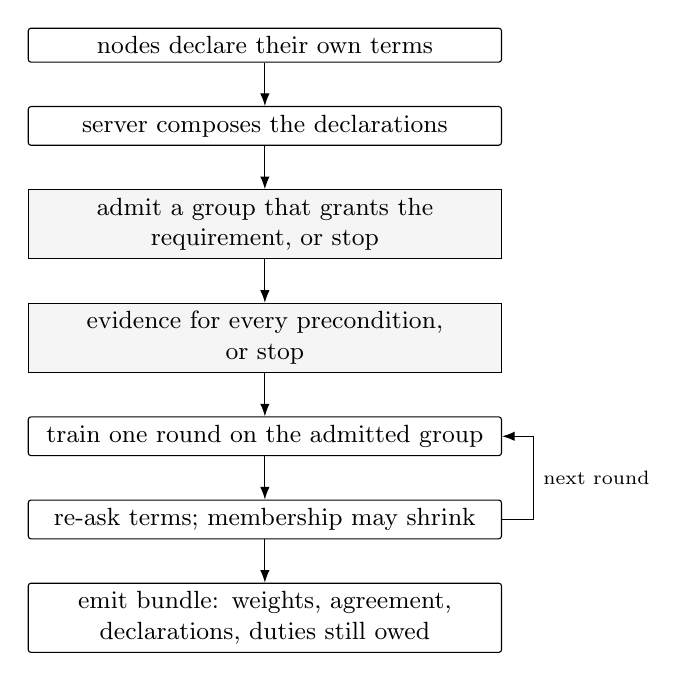
\begin{tikzpicture}[
  node distance=5.5mm,
  box/.style={draw, rounded corners=1pt, align=center, font=\small,
              inner sep=3pt, text width=58mm},
  dec/.style={draw, align=center, font=\small, inner sep=3pt,
              text width=58mm, fill=black!4},
  arr/.style={-{Latex[length=1.6mm]}},
]
\node[box] (declare) {nodes declare their own terms};
\node[box, below=of declare] (compose) {server composes the declarations};
\node[dec, below=of compose] (admit) {admit a group that grants the\\
  requirement, or stop};
\node[dec, below=of admit] (gate) {evidence for every precondition,\\
  or stop};
\node[box, below=of gate] (train) {train one round on the admitted group};
\node[box, below=of train] (recheck) {re-ask terms; membership may shrink};
\node[box, below=of recheck] (bundle) {emit bundle: weights, agreement,\\
  declarations, duties still owed};

\draw[arr] (declare) -- (compose);
\draw[arr] (compose) -- (admit);
\draw[arr] (admit) -- (gate);
\draw[arr] (gate) -- (train);
\draw[arr] (train) -- (recheck);
\draw[arr] (recheck) -- (bundle);
\draw[arr] (recheck.east) -- ++(4mm,0) |- node[pos=0.25, right, font=\scriptsize]
  {next round} (train.east);
\end{tikzpicture}
\caption{The policy round, the training loop and the bundle.}
\label{fig:pipeline}
\end{figure}

\subsection{The Fragment}

We work with a fragment of ODRL in which a policy is a set of rules over an
asset. A rule is a permission, a prohibition or a duty, each naming an action,
and each optionally carrying constraints. A constraint restricts an action to a
set of values of some operand, with the two we rely on being purpose and
location. Actions themselves are drawn from a small vocabulary, of which the
ones that matter for training are \emph{use}, \emph{aggregate} and
\emph{derive}, the last distinguishing a model that is a transformation of the
data from one that merely summarises it.

Purposes form a hierarchy and not a flat list. A permission granted for
\emph{research} covers \emph{ds-cancer}, because cancer research is research,
but the converse does not hold. The relation matters to composition because two
contributors granting different but related purposes are not in conflict: the
group may act for whatever purpose both grants cover, This is the more specific
of the two. Treating purposes as opaque strings reports conflicts that do not
exist, and in our measurements it changes the results.

\subsection{Composition}

The composition of a set of contributor policies is a single agreement, computed
element by element. Permissions intersect, because performing an action requires
every contributor's grant. Prohibitions are unioned, because a single
prohibition binds the entire group. Duties are likewise unioned and merged per
action, so that the strictest obligation applies. Constraints are conjoined,
through a set meet over a subsumption hierarchy or an interval intersection.
Conflicts are resolved by letting denial override. Table~\ref{tab:rules}
summarises the rules; the point to notice is that every one of them narrows.

\begin{table}[t]
\caption{Composition rules. Every rule narrows.}
\label{tab:rules}
\centering
\begin{tabular}{ll}
\toprule
Element & Rule \\
\midrule
Permissions & intersect: an action needs every contributor's grant \\
Prohibitions & union: one prohibition binds the whole group \\
Duties & union, merged per action: the strictest applies \\
Constraints & conjoin: set meet, or interval intersection \\
Conflict & deny overrides \\
\bottomrule
\end{tabular}
\end{table}

\subsection{Anti-Monotonicity}

Write $A(S)$ for the agreement composed from the policies of a contributor set
$S$, and $\mathrm{Cap}(S)$ for the set of actions the group may perform under
$A(S)$. The property the system rests on is that for contributor sets
$S \subseteq S'$,
\[
\mathrm{Cap}(S') \subseteq \mathrm{Cap}(S).
\]

The argument follows from the rules. Since permissions intersect, an action
permitted by $A(S')$ is permitted by every member of $S'$ and therefore by every
member of $S$. Prohibitions and duties only accumulate, and constraints only
narrow, so nothing in $A(S')$ can admit an action that $A(S)$ forbids.
Admitting a contributor can therefore never widen what the group may do with the
resulting model, however permissive that contributor is, and removing one can
never narrow it.

Two consequences matter for a system. The first is that a group which cannot
satisfy a requirement cannot be rescued by recruitment, so a server that has
found a candidate inadmissible need never reconsider it as a subset of
something larger. The second is that the family of admissible groups is
downward closed. That is exactly the condition under which candidate generation
in the style of Apriori~\cite{apriori} is sound. Candidates of size $k+1$ need
only be formed from admissible candidates of size $k$, and the remainder of the
space can be discarded without ever being examined. This is what can make a
search over the powerset affordable, and whether it does so depends on how much
there is to prune.

Algorithm~\ref{alg:admit} states the search. Line~\ref{alg:prune} is where
anti-monotonicity does the work. Without it, the loop would have to consider
every one of the $2^{n}-1$ subsets. How much it saves in practice depends on
how strict the requirement is, and we measure that in
Section~\ref{sec:pruning}.

\begin{algorithm}[t]
\caption{Admission by downward-closed search}
\label{alg:admit}
\begin{algorithmic}[1]
\Require declarations $D$, requirement $r$
\Ensure the largest admissible group, or none
\State $F_1 \gets \{\,\{d\} : d \in D,\ \mathrm{grants}(d, r)\,\}$
\State $k \gets 1$;\quad $best \gets \emptyset$
\While{$F_k \neq \emptyset$}
  \State $best \gets$ any member of $F_k$ of greatest data volume
  \State $C_{k+1} \gets \{\,S \cup S' : S, S' \in F_k,\ |S \cup S'| = k+1\,\}$
  \ForAll{$S \in C_{k+1}$} \label{alg:prune}
    \If{some $k$-subset of $S$ is not in $F_k$}
      \State discard $S$ \Comment{no superset can be admissible}
    \EndIf
  \EndFor
  \State $F_{k+1} \gets \{\,S \in C_{k+1} : \mathrm{grants}(A(S), r)\,\}$
  \State $k \gets k+1$
\EndWhile
\State \Return $best$
\end{algorithmic}
\end{algorithm}

We prove the property and we also test it in the implementation, using
property-based testing over randomly generated policies. The system relies on
the implementation and not on the proof.

\subsection{A Worked Example}
\label{sec:worked}

It is worth following the three contributors of
Section~\ref{sec:intro} through the algebra, because the outcome is easier to
accept once seen in the concrete. Each one declares a permission to
\emph{derive} its data, constrained to a set of purposes. Contributor~A
declares the following.

\begin{lstlisting}[style=jsonld]
{ "@context": "http://www.w3.org/ns/odrl.jsonld",
  "uid": "urn:policy:contributor-a",
  "permission": [{
    "target": "urn:asset:a",
    "action": "derive",
    "constraint": [{
      "leftOperand": "purpose",
      "operator": "isAnyOf",
      "rightOperand": ["ds-cancer", "method-dev"] }] }] }
\end{lstlisting}

Contributor~B declares the same shape with purposes
\texttt{["ds-neuro", "method-dev"]}, and contributor~C with
\texttt{["ds-cancer", "ds-neuro"]}. Now compose them, element by element, using
the rules of Table~\ref{tab:rules}. All three grant \emph{derive}, so the
intersection of the permitted actions keeps it. The purpose constraints are
conjoined, which for a set-valued operand is an intersection:
\[
\{\text{cancer},\text{method}\} \cap
\{\text{neuro},\text{method}\} \cap
\{\text{cancer},\text{neuro}\} = \emptyset .
\]

The permission survives with an unsatisfiable constraint, so the group may
\emph{derive} for no purpose at all. The composed agreement grants nothing, and
the three institutions cannot train a usable model together.

Any two of them can. A and B share \emph{method-dev}, A and C share
\emph{ds-cancer}, and B and C share \emph{ds-neuro}. A server that checked each
candidate on its own against its research question would therefore accept all
three, and would be wrong. This is the non-transitivity of
Section~\ref{sec:intro}, and it is why Algorithm~\ref{alg:admit} searches over
subsets instead of filtering members one at a time.

The example also shows why the purpose hierarchy matters. Suppose contributor~A
had declared \emph{research} instead of \emph{ds-cancer}. Compared as strings,
\emph{research} and \emph{ds-cancer} do not match, and composition would report
a conflict. Compared as classes of an ontology, cancer research is a kind of
research, so the meet of the two is \emph{ds-cancer} and the group retains a
purpose it really does hold.

%% ===========================================================================
\subsection{A Policy-Aware Federated Learning Server}
\label{sec:system}

The mechanism is implemented as a strategy for Flower, and it replaces the
participant sampling of federated averaging. We describe it in the order in
which the server executes it, because that ordering is the design. Each step
has to happen before something that would otherwise be impossible to undo.

\paragraph{Declarations Come from the Contributors}

The server could look up its clients' terms in a registry, and that would be
simpler, but a server that supplies its clients' consent terms demonstrates
nothing. Each node therefore translates its own conditions locally and declares
the result, and the server only ever acts on what it was told. A declaration is a small record. It carries the node's policy, the actions that policy grants, and the volume of data the node holds. The server parses it defensively. A missing policy, a malformed one, or one that is valid JSON but not a policy is rejected with a reason, and never treated as permissive.

That a declaration may be false is worth addressing directly, because it decides
whether the trust model is sound. Overstating a restriction only shrinks what
the declaring party may itself do with the group's model, so there is no
incentive to do it; understating one exposes the declaring party to the
consequences of a use it did not permit. Declared permissions are thus self-penalising. That is why they can be acted on at face value. This argument
does not extend to anything else a contributor might declare, and in particular
not to data quality, where the incentive runs the other way. We therefore ask
contributors to declare nothing except their terms.

\paragraph{Membership Is Decided Before Round One}

The server states what the federation must be able to do, as a set of required
actions and, importantly, a required purpose. The requirement is what makes the
check bite: a request naming only actions is granted by nearly every
contributor, so almost nobody is excluded and the mechanism demonstrates
nothing. With a purpose named, admission searches for a group whose composed
agreement grants the requirement, using the pruning of
Section~\ref{sec:algebra}, and returns both the admitted set and a reason for
each exclusion.

Two choices here are deliberate. First, admission is a pure function, kept separate from the strategy that honours it. This means it can be tested without starting a federation, and our test suite exercises it in isolation. That matters in practice, because the simulation backend is not available on every platform we develop on. And when
nothing is admissible the server fails. It does not fall back to training on everyone, because the fallback produces precisely the unusable model the
mechanism exists to prevent.

\paragraph{Obligations That Training Cannot Discharge}

Composition accumulates duties, and some of them are preconditions: an
obligation to obtain ethical approval before use cannot be discharged by the
run that depends on it. A system has one faithful option: to refuse to start without evidence that somebody discharged the obligation out of band. The
server therefore gates on evidence supplied as part of its configuration.
Nothing validates that the evidence is genuine, and it is not meant to: the
point is that a person has to assert it explicitly, so that the assertion is
recorded in the run's configuration and in the bundle the run produces.

\paragraph{Consent Is Not Settled Once}

Between rounds the server re-asks every active node for its terms and drops
those that have withdrawn, lapsed, or breached a duty too often. Membership can
therefore shrink during a run. The contribution set cannot, because a round that
has happened cannot be unhappened, and the resulting model remains a derivative
of every node that ever contributed to it. The bundle records both. That is the only honest way to represent a federation whose membership changed: the rights
attached to the model are composed from everyone who contributed, not from
whoever was still present at the end.

\paragraph{The Model Carries Its Agreement}

The run writes the weights alongside the composed agreement, every
contributor's declaration, and what remains owed. Two properties of this are
worth stating. Verification recomputes the agreement from the recorded declarations instead of comparing a stored hash, so a bundle whose agreement
does not follow from its declarations is detected and not trusted. And
composition is recursive: when the model is reused as a contribution to
something else, its agreement composes in like any other policy, so by
anti-monotonicity the rights attached to the result can only narrow. A
restricted model cannot be laundered into an unrestricted one by being used as
an ingredient.

The bundles are not signed, which we return to in
Section~\ref{sec:discussion}.

%% ===========================================================================
\subsection{Two-Stage Member Selection}
\label{sec:twostage}

\paragraph{Why a Second Stage Is Needed}

The policy filter is sound and incomplete. It decides admissibility exactly, and
it has nothing to say about which admissible group produces the better model. In
our measurements the filter typically leaves several hundred admissible
candidates out of a thousand, so the question it leaves open is not a small one.

The obvious response is to estimate utility without training, and we tried
three ways of doing so. A \emph{coverage} estimator scores a group by how much
of the label space its members jointly hold. A \emph{divergence} estimator
scores the Jensen--Shannon divergence between the group's pooled label
distribution and the uniform one. A \emph{gradient} estimator, the novel one, scores the coherence of the members' local gradients at a shared
initialisation, on the reasoning that clients whose gradients agree should
average well. All three fail, and Section~\ref{sec:eval} reports how. The
failure is not a side note: it is why the second stage trains.

\paragraph{Ranking by a Short Run}

The second stage trains every admissible candidate for a small number of rounds,
ranks them by the accuracy reached, and continues only the leaders to the full
budget. Three parameters describe it: the exploratory budget $R$, the shortlist
width $k$, and the total budget $T$. The cost in rounds is
\[
n R + k (T - R),
\]
where $n$ is the number of admissible candidates, against $nT$ for training
everything to completion. The first term dominates. That is the sense in which
the two stages depend on each other: the policy filter is what makes $n$ small
enough for the second stage to be affordable.

What the second stage recovers has to be stated carefully, and we return to it
with measurements in Section~\ref{sec:eval}. A short run does not identify the
best candidate. It identifies a near-optimal one, for a reason that is a property of the training curves and not of the ranking: by the point at
which the shortlist becomes reliable, the top of the field has flattened, so
ordering the leaders wrongly costs very little final accuracy. The engineering
claim is therefore that a short run separates bad candidates from good ones
dependably and good from best unreliably, and that this is sufficient when the object is a usable model and not an argmax.

%% ===========================================================================
\section{Proof of Concept}
\label{sec:eval}

\subsection{Experiment Design}

Measuring what a selection strategy gives up requires knowing what it could have
achieved, which means a ground truth that is exact and not sampled. We
therefore train \emph{every} non-empty subset of a ten-contributor pool, 1023 of
them, at each of 20 independently generated federations, for twenty rounds, and
record the whole accuracy curve of every run. A complete lattice means that a
statement such as ``this strategy missed the best candidate'' is a fact rather
than an artefact of which subsets happened to be drawn.

Each of those runs is repeated five times, varying only the training
randomness and holding the federation fixed. That is 102\,300 runs in total.
The replicates are not for error bars. Without them a strategy would be scored
against the single training run that it also selected on, so the best observed
candidate would partly be whichever one drew the kindest initialisation, and
every strategy's regret would be measured against that lucky draw. We instead
select on one replicate and score on the mean of the others, which makes the
comparison a held-out one. Section~\ref{sec:discussion} reports how much the
figures moved when we did this; the answer is a factor of four, and in the
direction that makes an unreplicated study look better than it is.

The task is a classification problem over synthetic Gaussian mixtures, split
across clients by a Dirichlet label skew at $\alpha = 0.3$. The skew is not
incidental. At $\alpha = 1.0$ every consortium converges to around 0.98 and the
spread across them is 0.005, which leaves no utility axis to estimate at all;
real institutions specialise, and a group missing a class cannot learn it.
We use twenty rounds and not five, because at five the task has not converged,
and an accuracy measured there reports how fast a group starts, and not how good its model is. Contributor policies are generated from the distribution of
condition sets observed in a public archive of real data use conditions.

Evaluation uses a shared held-out test set, never the contributors' own splits,
because scoring a group on its own data makes utilities incomparable across
groups: a single client holding two of four classes would be tested only on
those two and would out-score the full federation.

Sweeps run through an in-process implementation of federated averaging rather
than through the Flower transport, because comparing hundreds of candidate
groups means standing up hundreds of federations for models that train in under
a second, and the orchestration would dominate both the runtime and the failure
modes. Both paths report the same metric, and
Section~\ref{sec:eval} shows that they agree numerically on a federation run
through each.

\subsection{Results and Main Observations}

\paragraph{How far the pruning gets}
\label{sec:pruning}
Section~\ref{sec:algebra} argues that anti-monotonicity makes the search over
subsets affordable. Table~\ref{tab:pruning} measures it. Nothing is trained
here, because the search is a computation over declared terms, so we can reach
pool sizes at which training every subset would take weeks. Utility is the
number of members, deliberately: pruning is driven by feasibility and never by
utility, so a trivial utility keeps the result independent of how utility is
estimated.

\begin{table}[t]
\caption{Candidates examined before admission is decided.}
\label{tab:pruning}
\centering
\begin{tabular}{lrrrrr}
\toprule
Requirement & $n$ & $a$ & Subsets & Examined & Time \\
\midrule
\multicolumn{6}{l}{\emph{on the Flower server, instrumented}} \\
\emph{ds-cancer} & 4 & 2 & 15 & 5 & 0.004\,s \\
\emph{ds-cancer} & 8 & 5 & 255 & 34 & 0.015\,s \\
\emph{ds-cancer} & 16 & 12 & 65\,535 & 4\,099 & 3.2\,s \\
\emph{ds-cancer} & 24 & 18 & 16\,777\,215 & 262\,149 & 326\,s \\
\emph{ds-cancer} & 32 & --- & $4{\times}10^{9}$ & --- & $>$4\,h \\
\midrule
\multicolumn{6}{l}{\emph{offline, five corpora each}} \\
actions only & 16 & 13.8 & 65\,535 & 25\,634 & 23.3\,s \\
actions only & 17 & 15.5 & 131\,071 & 80\,005 & 86.1\,s \\
\emph{research} & 16 & 9.0 & 65\,535 & 889 & 0.5\,s \\
\emph{research} & 22 & 12.4 & 4\,194\,303 & 7\,586 & 8.1\,s \\
\bottomrule
\end{tabular}
\end{table}

The answer depends on the requirement, and in a way that has an exact form. The
instrumented server records the candidates it evaluated on every run, and over
four populations those counts are reproduced exactly by
\begin{equation}
\label{eq:cost}
\textrm{evaluated} \;=\; 2^{a} + (n - a) - 1 ,
\end{equation}
where $n$ is the number of contributors that declared and $a$ the number
admitted. Table~\ref{tab:pruning} gives the four measurements. The search
evaluates every subset of the admissible set, plus one probe for each
contributor that failed on its own terms, and nothing else.

Equation~\ref{eq:cost} says what the pruning does and does not achieve. It does
not make an exponential problem polynomial. It replaces the exponent: the cost
is exponential in the size of the \emph{admissible} set and not in the size of
the population. A requirement that admits everybody gives $a = n$ and saves
nothing at all. A requirement that admits few contributors is cheap however
large the federation becomes.

This explains the three regimes of the offline sweep without any further
appeal to intuition. Under \emph{research}, which is the broadest purpose and
therefore the hardest to satisfy, around nine contributors are admissible out
of sixteen, and the search examines 889 of 65\,535 subsets in half a second; at
a pool of 22 it examines 7\,586 of 4.19 million in 8.1\,s. Under a requirement
naming actions and no purpose, nearly everybody grants \emph{use} and
\emph{aggregate}, so $a$ approaches $n$ and the search gives up at 17
contributors after 86\,s.

The claim that cost follows $a$ and not $n$ can be tested directly, by
comparing configurations that share an admissible set size while differing in
population and in requirement. Two such pairs are present in our measurements,
and they are the strongest evidence we have for
Equation~\ref{eq:cost}.

A population of 13 under the weakest requirement admits 11.2 on average and
examines 3\,756 candidates in 3.5\,s. A population of 20 under \emph{research}
admits 11.6 and examines 3\,899 in 3.3\,s. Likewise a population of 14 under
the weakest requirement admits 12.0 and examines 7\,136, while a population of
21 under \emph{research} admits 12.2 and examines 7\,176. In both pairs the
populations differ by seven contributors, so the nominal search space differs
by a factor of 128, and the requirements differ as well. The measured cost
differs by 4\% in the first pair and by 1\% in the second. Across a
128-fold change in the size of the space being searched, the work is the same
to within a few per cent, because the admissible set is the same size.

Equation~\ref{eq:cost} also predicts where the method stops, which is more
useful than observing it. At 24 contributors the server admitted 18 and
evaluated 262\,149 candidates in 326\,s, a rate of 803 compositions per second
that agrees with the 893 per second measured offline. Extrapolating the same
admission rate to a population of 32 gives $a \approx 24$, hence 16.8 million
compositions and about 5.8 hours. Our 32-node run was stopped by a four-hour
scheduler limit while it was still searching, which is what
Equation~\ref{eq:cost} says should have happened. We did not repeat it with a
longer limit. The quantity it would confirm is already fixed by four exact
measurements and by the paired comparison above, and a population of 32 under a
narrower requirement is reached in minutes.

We draw the practical conclusion, and not the pessimistic one. The policy check
is affordable exactly when the federation's purpose is specific, and a
federation whose requirement names no purpose is one where the check has little
to decide. A consortium assembled to study one disease is both the realistic
case and the case the search handles best. Where it is not affordable, the
server knows so in advance: $a$ is the count of contributors that pass the
singleton test, which costs $n$ compositions, so Equation~\ref{eq:cost} can be
evaluated before the expensive stage begins.

Two limitations of the table. The offline rows at 17 and 18 contributors
average two generated corpora instead of five, because the sweep stops a
requirement once a single search runs long, so their times are less stable than
the others. And Equation~\ref{eq:cost} is an exact fit to four measurements,
not a proof. It follows naturally from a downward-closed search over an
admissible set, and we state it as a measured regularity.

\paragraph{The cost of ignoring policy}

We first ask what a policy-blind server gives up, against a baseline that
reflects how federations are actually assembled: take the contributors with the
most data. Table~\ref{tab:blind} reports, over a pool of sixteen contributors
and three requirements of increasing strictness, how often the group so chosen
is permitted to use the model it produced.

\begin{table}[t]
\caption{A policy-blind server against three requirements.}
\label{tab:blind}
\centering
\begin{tabular}{lrrr}
\toprule
Requirement & Blind group admissible & Search pruned \\
\midrule
actions only & 20\% & 60.9\% \\
\emph{ds-cancer} & 0\% & 83.7\% \\
\emph{research} & 0\% & 98.6\% \\
\bottomrule
\end{tabular}
\end{table}

Under the weakest requirement, which names actions but no purpose, the
volume-ranked group may use its own model one time in five. Once a purpose is
named it never may. The number to take from this is not the 20\%, which depends
on the requirement, but the asymmetry: the check that avoids the outcome costs
no training whatsoever, and it removes between 61\% and 98.6\% of the candidate
space as a side effect. That smaller set is what the second stage runs on.

The broader requirement prunes more. This deserves a moment's thought, because
it inverts the obvious expectation. A grant covering all of \emph{research} also
covers \emph{ds-cancer}, so requiring \emph{research} is the harder demand and
fewer groups meet it. Strictness in the requirement and breadth in the purpose
run in opposite directions.

\paragraph{Three estimators that do not work}

Table~\ref{tab:estimators} reports the three training-free estimators against
the exhaustive truth, restricted to the admissible candidates, since an
inadmissible group has no deployable utility however well it trains.

\begin{table}[t]
\caption{Training-free utility estimators over 20 federations.}
\label{tab:estimators}
\centering
\begin{tabular}{lrrr}
\toprule
Estimator & Kendall $\tau$ & Members picked & Regret \\
\midrule
coverage & 0.325 & 8.6 & 0.0231 \\
divergence & 0.435 & 8.6 & 0.0239 \\
gradient & $-0.144$ & 5.0 & 0.0769 \\
\bottomrule
\end{tabular}
\end{table}

All three cost real accuracy, with intervals excluding zero, and the pattern of
how they fail is more informative than the magnitude. The first two select 8.6
members where the best consortium has 4.0: both score a group monotonically in
its membership, so their maximum is always close to the largest admissible set,
and the decision they implement is in effect ``admit everyone you may''. The third, the novel one, anti-correlates with accuracy. We read that as
gradient coherence at initialisation measuring how similar clients are rather
than how much they jointly add, so that it rewards redundancy — which is the
opposite of what a heterogeneous federation needs.

Two caveats belong with this table and not in a footnote. Frontier recall
and precision, which we had intended as the primary measure, are not
interpretable here: 16 of the 20 federations are saturated, so which candidates
are non-dominated is settled by noise and not by the estimator, and the evaluation script reports this instead of printing a number. And the regret
column is measured against the best observed candidate without a held-out
replicate, so unlike Table~\ref{tab:costfidelity} it still carries the upward
bias of an argmax and is an upper bound on estimator error. The two columns are
therefore not directly comparable, and we rely on $\tau$ and the pick size for
the conclusion.

We report this, and we did consider leaving it out, for two reasons. It is the justification
for a second stage that trains. That is a design decision a reader would
otherwise question. And ``admit every contributor you are permitted to'' is a
strategy a practitioner might plausibly adopt on intuition, so it is worth
knowing what it costs: measured properly, as the largest-admissible row of
Table~\ref{tab:costfidelity}, 1.72 percentage points of accuracy against 0.09
for the full budget.

\paragraph{What a short run buys}

Every strategy is evaluated on the same twenty federations, so the comparison
between exploratory budgets is paired and the per-federation differences are
what we report. Regret is bounded below by zero and most federations sit near
that bound, so we give a bootstrap percentile interval on the mean difference instead of a symmetric one.

Table~\ref{tab:costfidelity} reports the second stage against the full budget
at a shortlist of three. The verdict column distinguishes three cases, and the
distinction is the result. A budget is \emph{worse} when the interval on the
difference excludes zero. It is \emph{equivalent} when the interval lies
entirely within the full budget's own regret, which says the shorter budget
differs from the full one by less than the full one differs from the truth. It
is \emph{cannot tell} when the interval contains zero but reaches beyond that margin. Such an interval tells us about our study, and not about the budget.

%% Generated from results/shortlist.csv. Do not edit by hand.
\begin{figure}[t]
\centering
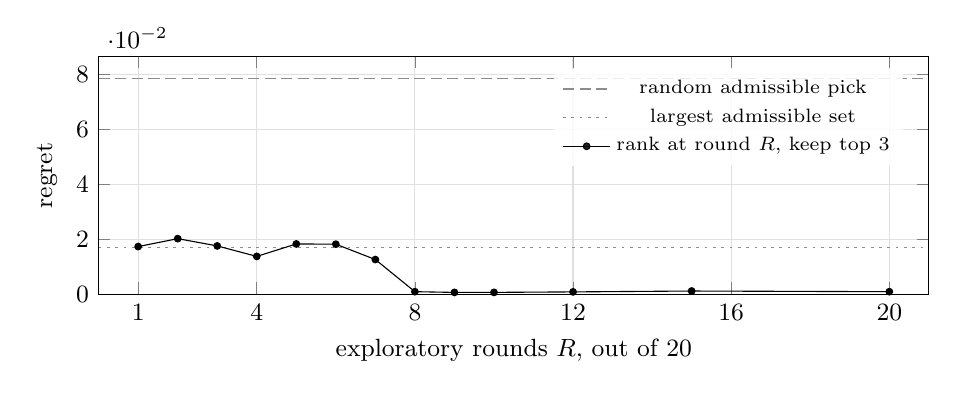
\begin{tikzpicture}
\begin{axis}[
  width=\columnwidth, height=46mm,
  xlabel={exploratory rounds $R$, out of 20},
  ylabel={regret}, ylabel near ticks,
  xmin=0, xmax=21, ymin=0,
  xtick={1,4,8,12,16,20},
  label style={font=\small}, tick label style={font=\small},
  legend style={font=\scriptsize, at={(0.97,0.95)},
    anchor=north east, draw=none, fill=white,
    fill opacity=0.85, text opacity=1},
  grid=major, grid style={black!12},
]
\addplot[black!45, dash pattern=on 4pt off 2pt, no markers] coordinates {(0,0.078668) (21,0.078668)};
\addlegendentry{random admissible pick}
\addplot[black!45, dash pattern=on 1pt off 2pt, no markers] coordinates {(0,0.017162) (21,0.017162)};
\addlegendentry{largest admissible set}
\addplot[black, mark=*, mark size=1.2pt] coordinates {(1,0.017381) (2,0.020263) (3,0.017619) (4,0.013800) (5,0.018337) (6,0.018244) (7,0.012656) (8,0.000956) (9,0.000687) (10,0.000700) (12,0.000875) (15,0.001194) (20,0.000950)};
\addlegendentry{rank at round $R$, keep top 3}
\end{axis}
\end{tikzpicture}
\caption{Regret falls to the full budget's level by round eight.}
\label{fig:costfidelity}
\end{figure}


\begin{table}[t]
\caption{Short runs against the full budget, $k=3$.}
\label{tab:costfidelity}
\centering
\begin{tabular}{lrrl}
\toprule
Strategy & Regret & Cost & Difference from full budget \\
\midrule
random admissible & 0.0787 & --- & --- \\
largest admissible & 0.0172 & --- & --- \\
\midrule
round 1 & 0.0174 & 5.9\% & $[+0.0012, +0.0424]$ worse \\
round 4 & 0.0138 & 20.7\% & $[-0.0006, +0.0380]$ cannot tell \\
round 7 & 0.0127 & 35.6\% & $[-0.0006, +0.0359]$ cannot tell \\
round 8 & 0.0010 & 40.5\% & $[-0.0006, +0.0007]$ \textbf{equivalent} \\
round 10 & 0.0007 & 50.4\% & $[-0.0006, +0.0001]$ equivalent \\
\midrule
full budget & 0.0009 & 100\% & --- \\
\bottomrule
\end{tabular}
\end{table}

Two features of this table matter more than the regret column. The first is
that the full budget does not score zero. Because the shortlist is chosen from
one replicate and scored on the others, training every candidate and taking the
argmax is itself partly selecting on noise, and it gives up 0.0009. Kendall
$\tau$ between its ranking and the replicate-averaged truth is 0.866 rather
than 1, and the genuinely best candidate sits at rank 42. An exhaustive search
is a strategy here, not an oracle.

The second is where the structure lies. The mean differences wobble
non-monotonically between rounds three and seven, and none of those rows is
resolvable: at round seven the interval reaches to $+0.036$, forty times the
margin. What changes at round eight is not the mean but the precision. The
interval narrows from a width of 0.0366 to 0.0013, a factor of
twenty-nine, in one step. Below that point the study cannot tell whether a
short run costs anything; from it, the difference is smaller than the full
budget's own error.

The knee is therefore real and is a knee in the resolution of the comparison.
It sits at eight rounds for shortlists of one and three, and at nine for a
shortlist of five, which misses at eight by 0.00011. The margin also tightens
as the shortlist widens, from 0.00143 through 0.00095 to 0.00071, because a
wider shortlist improves the baseline and so raises the bar; that the
conclusion survives a moving bar is worth more than the bar's exact position.
``Around eight rounds'' is the honest phrasing.

One detail falls out in the right direction. At nine and ten rounds the mean
difference is negative, so ranking on a short run is if anything marginally
better than training everything and taking the argmax. It is not significant,
but it is what the selection bias predicts: a longer exploratory run fits the
selection replicate's noise more closely.

We also note what does \emph{not} explain the result. $\tau$ rises smoothly
from 0.240 to 0.866 with no break anywhere, so round eight is not where the
ranking becomes correct; at that point the ordering is still substantially
wrong and the best candidate sits at rank 33. The shortlist works because the
top of the field has flattened, not because it has been correctly sorted. The
number eight is a property of where this task's curves flatten. That is why we report a curve and expect a deployment to measure its own.

\subsection{The System in Operation}

The sweeps above establish what the mechanism decides. This section reports it
deciding, as a Flower simulation with a population of ten SuperNodes, under a
requirement naming the purpose \emph{ds-cancer}.

The server's own log of the policy round is the result:

\begin{quote}\small
\texttt{policy round: 10 nodes declared}\\
\texttt{admitted 7 of 10 declared}\\
\texttt{\ \ excluded node 1302686541 -- terms do not}\\
\texttt{\ \ compose with the selected consortium}\\
\texttt{\ \ excluded node 16554732426 -- \ldots}\\
\texttt{\ \ excluded node 18311162132 -- \ldots}\\
\texttt{the federation may: aggregate, derive,}\\
\texttt{\ \ distribute, use}\\
\texttt{before starting, must evidence: obtainConsent}\\
\texttt{OUTSTANDING inform -- owed by 7 contributors,}\\
\texttt{\ \ not dischargeable by training}
\end{quote}

Four things in that are worth drawing out. Membership was decided before the
first round, and not audited afterwards, and the three exclusions carry a
reason rather than being silent, which is what makes the decision reviewable.
The composed capability is reported explicitly, so what the resulting model may
be used for is written down as an output of the run. A reader does not have to work it
out later. The duty gate fired: the composed agreement requires
\emph{obtainConsent}, that obligation cannot be discharged by the run which
depends on it, and the server refused to train, raising
\texttt{UnmetPrecondition} before any round began. And one duty, \emph{inform},
is recorded as outstanding and explicitly not dischargeable by training, so it
travels in the bundle as something still owed by seven of the contributors.

The refusal is the behaviour we argued for in Section~\ref{sec:system} and we
report it as an observation rather than describing it, because a mechanism that
declines to start is only credible once it has been seen declining.

Supplying the evidence the gate asks for allows the run to proceed, and it then
completes: twenty rounds, seven results and no failures in every round, central
accuracy rising from 0.1945 at initialisation to 0.9930, and 22.4\,s of
strategy execution for the whole federation including the policy round. The run
ends by writing the bundle, whose manifest records the composed agreement, the
seven contributors it was built from, the four actions the holder may perform,
the cleared precondition with its evidence reference, and the one duty still
owed to all seven.

That last line is the part we would draw a reader's attention to. The artefact
leaves the system carrying an obligation, in a form that a later tool can read. It does not simply carry a note saying that an obligation existed.

\paragraph{Where the policy round spends its time}
The instrumented server separates two costs that are easy to conflate:
collecting the declarations, which is communication, and deciding admission,
which is computation. They behave completely differently.

Deciding admission grows as Equation~\ref{eq:cost} says, from 4\,ms at four
contributors to 326\,s at twenty-four. Collecting the declarations does not
grow at all. It takes 16.4\,s at four contributors and 14.1\,s at
twenty-four, so it is dominated by fixed start-up cost in the simulation
backend and not by the number of nodes being asked. A declaration is about
1.4\,kB, with the largest we observed at 2.9\,kB, so the whole policy round
moves roughly 32\,kB at a population of twenty-four.

The cost of the policy round is therefore computational and not
communicational. That is the opposite of what one might assume about a step
whose first action is to ask every node a question, and it says where to look
if the round ever needs to be made faster.

\paragraph{The two paths agree}
Section~\ref{sec:eval} runs its sweeps in process and not over the Flower transport, so the two must be shown to compute the same thing. The admitted
consortium of this run is one of the 1023 in the lattice, at the same
heterogeneity and seed, which makes the comparison a lookup rather than a
further experiment. The Flower path reaches 0.9930 and the in-process path
0.9935, a difference of one test example in two thousand, and the per-round
curves track each other throughout with a largest mid-curve gap of 0.011. They
are not bit-identical, and should not be expected to be: the runs execute in
different orders across Ray workers and, as noted below, under different
releases of the tensor library. Agreement to five parts in ten thousand is what
the comparison needs.

\paragraph{What this run does not show}
The federation it ran on is a saturated one. At that seed the median subset
reaches 0.9945 and 889 of the 1023 subsets exceed 0.99, so accuracy barely
discriminates between consortia there and the 0.9930 above should not be read
as evidence that the admitted seven were a good choice. It is evidence that the
mechanism runs, admits, gates, trains and emits a bundle. Which consortium is
better is the question Section~\ref{sec:eval} answers across twenty
federations, and the saturated ones are exactly the ones it has to set aside.

One methodological note belongs here, because it would otherwise invalidate the
comparison this section is for. Flower builds a separate runtime environment
for each run, resolved from the project's dependencies, so the Flower path and
the in-process sweeps can end up on different releases of the tensor library:
in our case 2.14.1 against 2.5.1, with a third version on the development
machine. We therefore checked this instead of assuming it, and all 5115 runs of the
smaller lattice are bit-identical across two of those versions. The task is a
small network over synthetic data with every seed fixed, and nothing in it
reaches an operation whose result moved between those releases. A study on a
larger model should not expect that and should pin the version.

%% ===========================================================================
\section{Discussion and Lessons Learnt}
\label{sec:discussion}

\subsection{What the Results Establish}

The combinatorial results are the firm ones, and they are firm because they
never touch a model, a metric or a dataset. Four of them matter. Capability is anti-monotone. Compatibility is not transitive. The resulting search is downward closed and can therefore be pruned. And a group ranked by data volume is usually not permitted to use its own model. All four follow from composing declared terms, and no choice of task, model or metric would change any of them.

The results about model quality are weaker and we would rather say so than
imply otherwise. They rest on a synthetic task, on one heterogeneity setting,
and on a pool of ten contributors chosen because $2^{10}$ subsets can be trained
exhaustively and $2^{16}$ cannot.

\subsection{Assumptions}

The mechanism assumes that contributors declare their terms truthfully, which
Section~\ref{sec:system} argues is sound because declared restrictions are
self-penalising. It assumes conditions are expressed in a vocabulary with a
subsumption hierarchy, since without one composition reports conflicts that do
not exist. And it assumes the contributors' data is of comparable quality,
because the mechanism observes conditions and not data: a contributor
combining permissive terms with poor data is invisible to it and would have to
be excluded by other means. The last of these is the strongest assumption in the
paper and the one we would most want to remove.

\subsection{Limitations}

Bundle manifests are not signed. A forger who rewrites the declarations and the
agreement consistently produces a bundle that verifies, and a test in our suite
asserts exactly that. This is tolerable for a study and disqualifying for a
deployed licensing mechanism; closing it needs signatures over the digest and a
key distribution story, for which the provenance work in C2PA is the obvious
prior art.

Regret is measured against the best candidate observed, and an argmax over
several hundred noisy candidates is biased upward, because the winner is partly
whichever candidate drew the kindest initialisation. Small groups vary more than
large ones against a flat ceiling, so the observed maximum is more often a lucky
small draw than a genuinely better group. Removing that bias needs replicate
training runs within each federation. That is roughly five times the compute,
and every figure above comes from such a campaign: 1023 candidates at 20
federations with five replicates each, 102\,300 training runs, with the
shortlist chosen from one replicate and scored on the mean of the others.

This changed the result instead of confirming it, which is the more useful
thing to report. Scored against its own training run the full budget had zero
regret by construction, the largest-admissible baseline 0.0697 and a random
admissible pick 0.1230. Scored against held-out replicates those become 0.0009,
0.0172 and 0.0787. The earlier numbers were not merely imprecise: the apparent
margin by which a short run beat nothing was partly the full budget being
compared against its own lucky draw, and the baselines were inflated by the
same amount. Any study of this kind that selects and scores on one training run
should expect its effect sizes to shrink by a similar factor.

What remains is a sample of twenty federations for a strongly skewed quantity.
That is enough to resolve the difference at eight rounds, where the interval is
narrower than the margin, and not enough to resolve it between three and seven,
where the intervals reach forty times the margin. We report those as
unresolved. We do not call them equivalent.

Finally, ``more contributors is better'' held in our setting, and it should not
be expected to hold in general. We measured it under uniform data quality and a
shared conditional distribution. Our task varies which labels each client
holds, and never what the correct answer is. Introduce variation in quality, or
a shift in the concept being learned, and monotonicity in the training signal
breaks. Anti-monotonicity in the policy signal does not break, because it is a
property of declared terms and not of data.

\subsection{Threats to Validity}

We group the threats by the kind of claim each one affects.

\emph{Construct validity.} Regret measures the accuracy given up against the
best candidate that was observed. It is the right quantity for a selection
procedure, and it is not a measure of how good the model is in absolute terms.
We also use capability, the set of actions a composed agreement permits, as our
measure of what a group may do. A richer measure might weight actions by their
value, and we do not attempt that.

\emph{Internal validity.} Two threats here, and we have addressed both. The
first is the selection bias discussed above, which replicate runs remove. The
second is saturation. In federations where nearly every candidate reaches the
same accuracy, any difference between selection strategies is decided by noise.
Our evaluation detects saturation and reports it, and 16 of the 20 federations
are saturated on the frontier measures. That is why we rely on rank
correlation and pick size for the estimator result.

\emph{External validity.} This is the weakest of the three. The task is
synthetic, at one heterogeneity setting, over a pool of ten contributors. We
chose ten because $2^{10}$ subsets can be trained exhaustively and $2^{16}$
cannot, and an exhaustive lattice is what makes a statement about the best
candidate a fact. The combinatorial results do not depend on any of this, since
they never touch a model. The results about model quality do, and we would not
expect the number eight to carry across to a different task.

\emph{Reliability.} Every number reported here is produced by a script from a
committed data file, and the figures and tables are generated from the same
files as the text. We also checked that the lattice reproduces across machines
and across releases of the tensor library. We report that with the system results above.

\subsection{Scope}

Although we implement and evaluate this in federated learning, most of the
mechanism is not specific to it. The algebra applies to any artefact derived
from several governed sources, whether a trusted research environment, a shared
analysis platform, or a model fine-tuned on pooled records, and nothing in the
composition rules refers to how training is distributed. Federated learning is
where the check becomes executable, because the participants' terms are already
declared to the system that coordinates them, so composition can happen before the first round, instead of being negotiated out of band. Centralising the data
would not avoid the problem either: the resulting model remains a derivative of
every source, the terms of every source continue to bind it, and the loss of
capability is unchanged by where the computation happens.

%% ===========================================================================
\section{Conclusion}
\label{sec:conclusion}

Conditions attached to data compose, and they compose in one direction only. We have presented a federated learning server that computes the composition before it allocates any compute. We proved that the capability it computes is anti-monotone in the contributor set. We then used that property to prune the search over candidate groups, so that the whole check fits in the time between a node connecting and the first round beginning. Because the check is sound and incomplete, we paired it with a second
stage that ranks the admissible candidates by a short exploratory run, and
measured what that costs against an exhaustively trained lattice of 102\,300
runs. Around eight of twenty rounds is \emph{equivalent} to training every
candidate to completion, in the sense that the paired difference between them is
smaller than the full budget's own distance from the truth, at two fifths of the
compute. One round is measurably worse, and between three and seven rounds
twenty federations cannot resolve the question.

The estimators are reported as a negative result because they are the reason the
second stage is shaped as it is, and because the heuristic they reduce to is one
a practitioner might reasonably choose. The asymmetry that makes the whole
design work is worth restating: permissions can be taken from a declaration,
since claiming more restrictions than one has only shrinks what one may do,
whereas data quality cannot be, because the incentive runs the other way.
Quality has to be measured, and the policy filter is what makes measuring it affordable, and not what makes it unnecessary.

Signing the bundle manifest is the open item that would turn a policy-carrying
model from a description into a mechanism, and removing the uniform-quality
assumption is the one that would make the second stage interesting and not merely cheap.

%% ---------------------------------------------------------------------------
\section*{Data Availability}

The implementation, the generated policy corpus, the exhaustive lattice and
every result table reported here are available at \repourl. All tables are
produced from committed result files, so every number above can be traced to
the run that produced it.

\bibliographystyle{IEEEtran}
\bibliography{refs}

\end{document}
